\documentclass[10pt,a4paper]{article}

\usepackage[utf8]{inputenc}
\usepackage[T1]{fontenc}
\usepackage[spanish]{babel}
\usepackage[margin=1.25cm,top=1.05cm,bottom=1.05cm]{geometry}
\usepackage{booktabs}
\usepackage{tabularx}
\usepackage{array}
\usepackage{graphicx}
\usepackage{xcolor}
\usepackage{enumitem}
\usepackage{caption}
\usepackage{amsmath}
\usepackage{hyperref}
\setlength{\parindent}{0pt}
\setlength{\parskip}{2pt}
\renewcommand{\arraystretch}{0.94}
\setlist[itemize]{nosep,leftmargin=1.2em}
\setlist[enumerate]{nosep,leftmargin=1.5em}
\captionsetup{font=footnotesize,skip=2pt}
\hypersetup{colorlinks=true,urlcolor=blue}
\newcolumntype{Y}{>{\raggedright\arraybackslash}X}
\newcommand{\smallsection}[1]{\vspace{2pt}\textbf{\large #1}\par\vspace{1pt}}

\begin{document}
\small
\begin{center}
{\LARGE\bfseries Auditoría de DARL DQN Dummy v4}\\[-1pt]
{\small Recorrido del notebook, oportunidades de A3 y diagnóstico del 95\%}
\end{center}
\vspace{-3pt}

\smallsection{Alcance y datos}
Se verificaron los bloques de código de \texttt{kaggle/dqn-dummy/v4/input/main.ipynb},
los ocho CSV del resultado principal y las gráficas usadas abajo. La corrida
registra 1\,552\,210 filas de PhysioNet/Computing in Cardiology Challenge 2019
y 40\,336 pacientes (Reyna et al., 2020). Las siete entradas son HR, O2Sat,
Temp, SBP, MAP, DBP y Resp. El objetivo de XGBoost es \texttt{y\_dummy}, una
etiqueta artificial construida con un score de vitales y ruido determinista
del 5\%; \texttt{SepsisLabel} solo estratifica las particiones. Por tanto, la
AUC de este ensayo no mide detección clínica de sepsis.

\smallsection{Notebook, de entrada a resultado}
\begin{tabularx}{\textwidth}{@{}p{0.24\textwidth}Y@{}}
\toprule
\textbf{Bloque / recibe} & \textbf{Proceso y produce} \\
\midrule
Carga y partición: parquet, patient\_id, ICULOS, signos vitales y SepsisLabel
& Ordena por paciente/tiempo, aplica forward-fill causal, separa pacientes
A (70/15/15) y B (60/20/20); cada segmento B se divide en pacientes de
actualización/evaluación. Construye \texttt{y\_dummy}. \\
Replay y pipeline: pacientes, días y roles
& Simula 200 camas (100 update, 100 eval) por 16 días. XGBoost inicial usa
60 árboles; mediana/IQR y clipping a \([-2,2]\). A1 no cambia; A2 recalibra
transformación; A3 reentrena XGBoost; A4 hace ambas cosas. \\
Drift y observación: replay y calendario
& \texttt{inject} desplaza los vitales (covariate), cambia la regla de
\texttt{y\_dummy} (concept), o aplica ambos. KS, PSI y AUC se cuantizan en
categorías; se concatenan las últimas tres observaciones (estado de 30 valores). \\
DQN, reward y evaluación
& Double DQN estima cuatro valores \(Q\) con una red 30--128--128--4,
epsilon-greedy, replay FIFO, Huber y red target. Al actuar el día \(d\),
la recompensa se revela con la AUC de evaluación en \(d+1\), menos costo
temporal normalizado. El retorno suma 15 recompensas válidas por episodio. \\
\bottomrule
\end{tabularx}

\smallsection{Una decisión completa: concept, día 7}
\textbf{Antes de elegir:} el estado de día 7 incluye KS \(=0{,}0687\),
PSI \(=0{,}0202\), AUC actual \(=0{,}8616\) y su historial categorizado.
Como KS/PSI están debajo de 0,10 y AUC encima de 0,85, la codificación todavía
representa señales bajas/altas aunque el concepto ya deriva (\(u=0{,}45\)).
Los valores almacenados fueron \(Q(A1)=1{,}5023\), \(Q(A2)=1{,}4581\),
\(Q(A3)=1{,}4218\), \(Q(A4)=1{,}4546\); greedy selecciona A1. Tras la decisión,
la AUC del día 8 cae a 0,8101; costo \(=0{,}000000664\), reward
\(=0{,}810063\).

\textbf{Lo que solo conoce la auditoría posterior:} calcula, fuera de la
política, las cuatro alternativas desde el mismo pipeline y datos de
actualización del día 7, y mide cada una sobre la evaluación del día 8.
Encuentra \(U(A3)=0{,}875907\), \(U(A1)=0{,}810063\) y regret
\(=0{,}065844\). El agente no recibe el oracle ni la AUC futura. \textbf{Cautela
temporal:} el código sí calcula la AUC de evaluación del día actual para
formar la observación antes de actuar; no implementa un retraso explícito de
esa etiqueta actual. Si el supuesto de tesis exige etiquetas retrasadas, hay
que corregir el entorno antes de presentar v4 como fiel a ese supuesto.

\smallsection{Oportunidades donde A3 fue el oracle de un paso}
\scriptsize
\begin{tabular}{@{}llrrrr@{}}
\toprule
\textbf{Escenario} & \textbf{Día} & \textbf{DQN} & \(\boldsymbol{U(A3)}\) &
\textbf{\(U\) elegida} & \textbf{Regret} \\
\midrule
concept & 6 & A1 & 0,8783 & 0,8616 & 0,0168 \\
concept & \textbf{7} & \textbf{A1} & \textbf{0,8759} & \textbf{0,8101} & \textbf{0,0658} \\
concept & 8 & A3 & 0,8792 & 0,8792 & 0,0000 \\
concept & 9 & A1 & 0,8855 & 0,8745 & 0,0110 \\
concept & 14 & A1 & 0,8821 & 0,8564 & 0,0257 \\
concept & 15 & A1 & 0,8943 & 0,8523 & 0,0420 \\
combined & \textbf{9} & \textbf{A2} & \textbf{0,8832} & \textbf{0,8371} & \textbf{0,0460} \\
combined & 10 & A4 & 0,8783 & 0,8703 & 0,0080 \\
combined & 12 & A2 & 0,8804 & 0,8378 & 0,0426 \\
combined & \textbf{13} & \textbf{A4} & \textbf{0,8862} & \textbf{0,8768} & \textbf{0,0094} \\
\bottomrule
\end{tabular}
\small
\vspace{2pt}

\textbf{Tres casos:} (1) Concept día 7: \(Q(A1)>Q(A3)\), pero la información
categorizada aún no refleja la caída suficiente; es la mayor de estas pérdidas.
(2) Combined día 9: \(Q(A2)=1{,}1358\) supera \(Q(A3)=1{,}0149\), así que el DQN
elige recalibrar features; el oracle inmediato favorece A3 por 0,0460.
(3) Combined día 13: el agente elige A4 (\(Q=0{,}9561\)); A3 supera su utilidad
solo por 0,0094. Es una diferencia pequeña y el regret queda bajo 0,01.
El oracle es de un paso, no una política óptima de horizonte largo.

\newpage
\smallsection{Métodos, comparadores y lectura de los CSV}
La partición por paciente evita repartir horas de una misma persona entre
ajuste y evaluación. Se comparan A1--A4, DQN, aleatoria y una heurística.
La heurística usa umbrales KS/PSI/AUC relacionados con los cortes de
observación; no debe describirse como acceso a señales distintas. A1 es el
control sin mantenimiento; A2 y A3 aíslan transformación/modelo; A4 es la
actualización completa. XGBoost es el modelo de clasificación
(Chen y Guestrin, 2016); DQN aprende valores de acción mediante Q-learning
profundo y Double DQN (Mnih et al., 2015; van Hasselt et al., 2016).

\scriptsize
\begin{tabularx}{\textwidth}{@{}p{0.25\textwidth}p{0.12\textwidth}Y@{}}
\toprule
\textbf{CSV} & \textbf{Filas} & \textbf{Hallazgo / límite} \\
\midrule
\texttt{actions.csv} & 420 & 60 acciones por cada una de 7 políticas; DQN registra acción solicitada/ejecutada, Q, AUC, costo y reward. \\
\texttt{action\_audit.csv} & 60 & Las cuatro utilidades y regret están presentes; oracle elige A3 10 veces; coincidencia exacta DQN--oracle 49/60 = 81,7\%. \\
\texttt{training\_history.csv} & 1000 & 100 validaciones (cada 10 episodios), epsilon, retorno y acuerdos; faltantes en episodios sin validación son esperados. \\
\texttt{policy\_comparison.csv} & 28 & 7 políticas \(\times\) 4 escenarios, 15 rewards válidos cada una; una semilla, sin intervalos de incertidumbre. \\
\texttt{calibration.csv} & 6 & 3 rates por tipo; 0,25 IQR/día y 0,15 unidades/día son los rates más lentos que califican. \\
\texttt{daily\_metrics.csv} & 448 & AUC completa en 16 días; 28 rewards faltantes corresponden al día terminal, sin acción siguiente. \\
\texttt{stage\_calendar.csv} & 64 & Cuatro rampas de 16 días; combined inicia covariate en día 5 y concept en día 7. \\
\texttt{drift\_dia1\_vs\_dia16.csv} & 2 & Resumen auxiliar de covariate/concept; KS día 1--16 mezcla inyección y recambio de cohortes. \\
\bottomrule
\end{tabularx}
\small

\textbf{Retorno A1/A2/A3 (y DQN):} covariate 11,794/13,776/12,606 (13,843);
concept 11,369/11,052/13,271 (13,382); combined 11,700/11,826/12,556 (13,467).
Los costos acumulados DQN son 0,097/0,095/0,164. En stable, DQN coincide con A1.
Una corrida no permite generalizar estadísticamente.

\textbf{Proveniencia gráfica:} el manifiesto declara 18 rutas (9 PNG + 9 SVG),
pero el directorio tiene 17 PNG y ningún SVG; incluye variantes 04a/b y 05a/b,
07a/b y dos figuras del notebook auxiliar. No asumir que son 18 pares exportados.

\smallsection{Estabilidad: evidencia, interpretación y próximo paso}
El gate exige variación del retorno \(\leq5\%\) y acuerdo exacto \(\geq95\%\).
v4 obtuvo 1,47\% y 85\% (51/60): pasó el primero y falló el segundo. Ningún
checkpoint alcanzó 95\% (máximo 90\%); los cinco finales fueron 35\%, 38\%,
87\%, 83\%, 85\%. Se agotaron 1000 episodios y 14\,937 actualizaciones.

No se demostró una causa única. La discretización puede retrasar concept:
en días 3--7, KS/PSI quedan bajo sus cortes y la AUC no cruza 0,85 hasta el día 8.
La política seleccionada es del episodio 940, pero el gate compara 990 con 1000;
85\% no mide estabilidad alrededor del checkpoint reportado. Siguiente paso:
medir checkpoints vecinos por escenario y varios bloques consecutivos, registrar
márgenes Q/regret, repetir semillas y mantener B-test intacto. Más episodios o
bajar el umbral no prueban convergencia.

\smallsection{Gráficas: observación, valores Q y entrenamiento}
\begin{center}
\begin{minipage}[t]{0.485\textwidth}
\centering
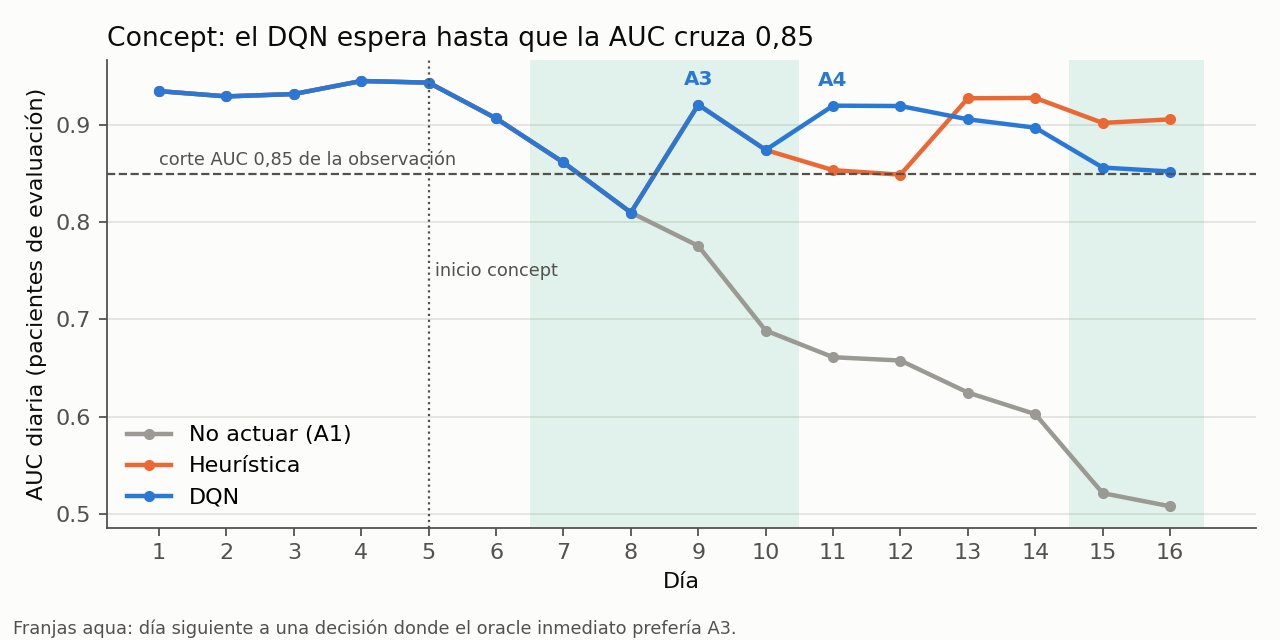
\includegraphics[width=\linewidth]{kaggle/dqn-dummy/v4/outputs/analisis/A_concept_auc_dqn_heuristica.png}
\captionof{figure}{Concept: el DQN selecciona A3 tras cruzar el corte de AUC 0,85. La trayectoria A1 sin acción cae; la franja verde identifica días posteriores a oportunidades oracle A3.}
\end{minipage}\hfill
\begin{minipage}[t]{0.485\textwidth}
\centering
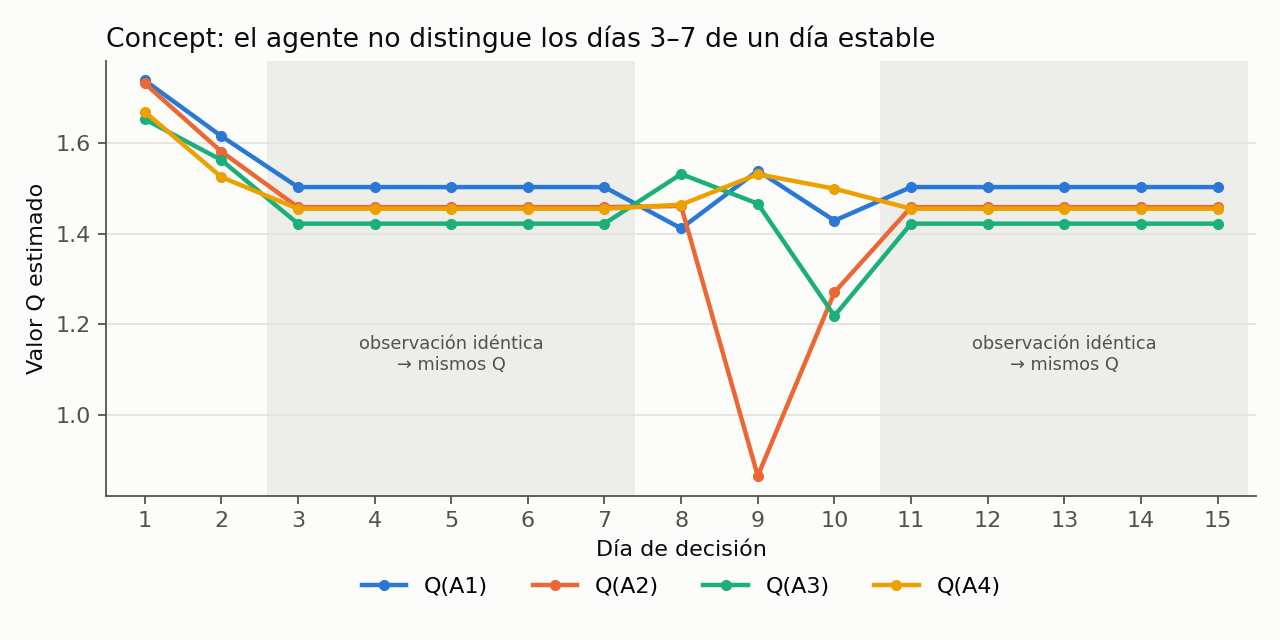
\includegraphics[width=\linewidth]{kaggle/dqn-dummy/v4/outputs/analisis/B_concept_valores_q.png}
\captionof{figure}{Los \(Q\) son iguales en días 3--7 porque las señales caen en las mismas categorías; en día 7 \(Q(A1)\) es mayor que \(Q(A3)\).}
\end{minipage}
\end{center}
\begin{center}
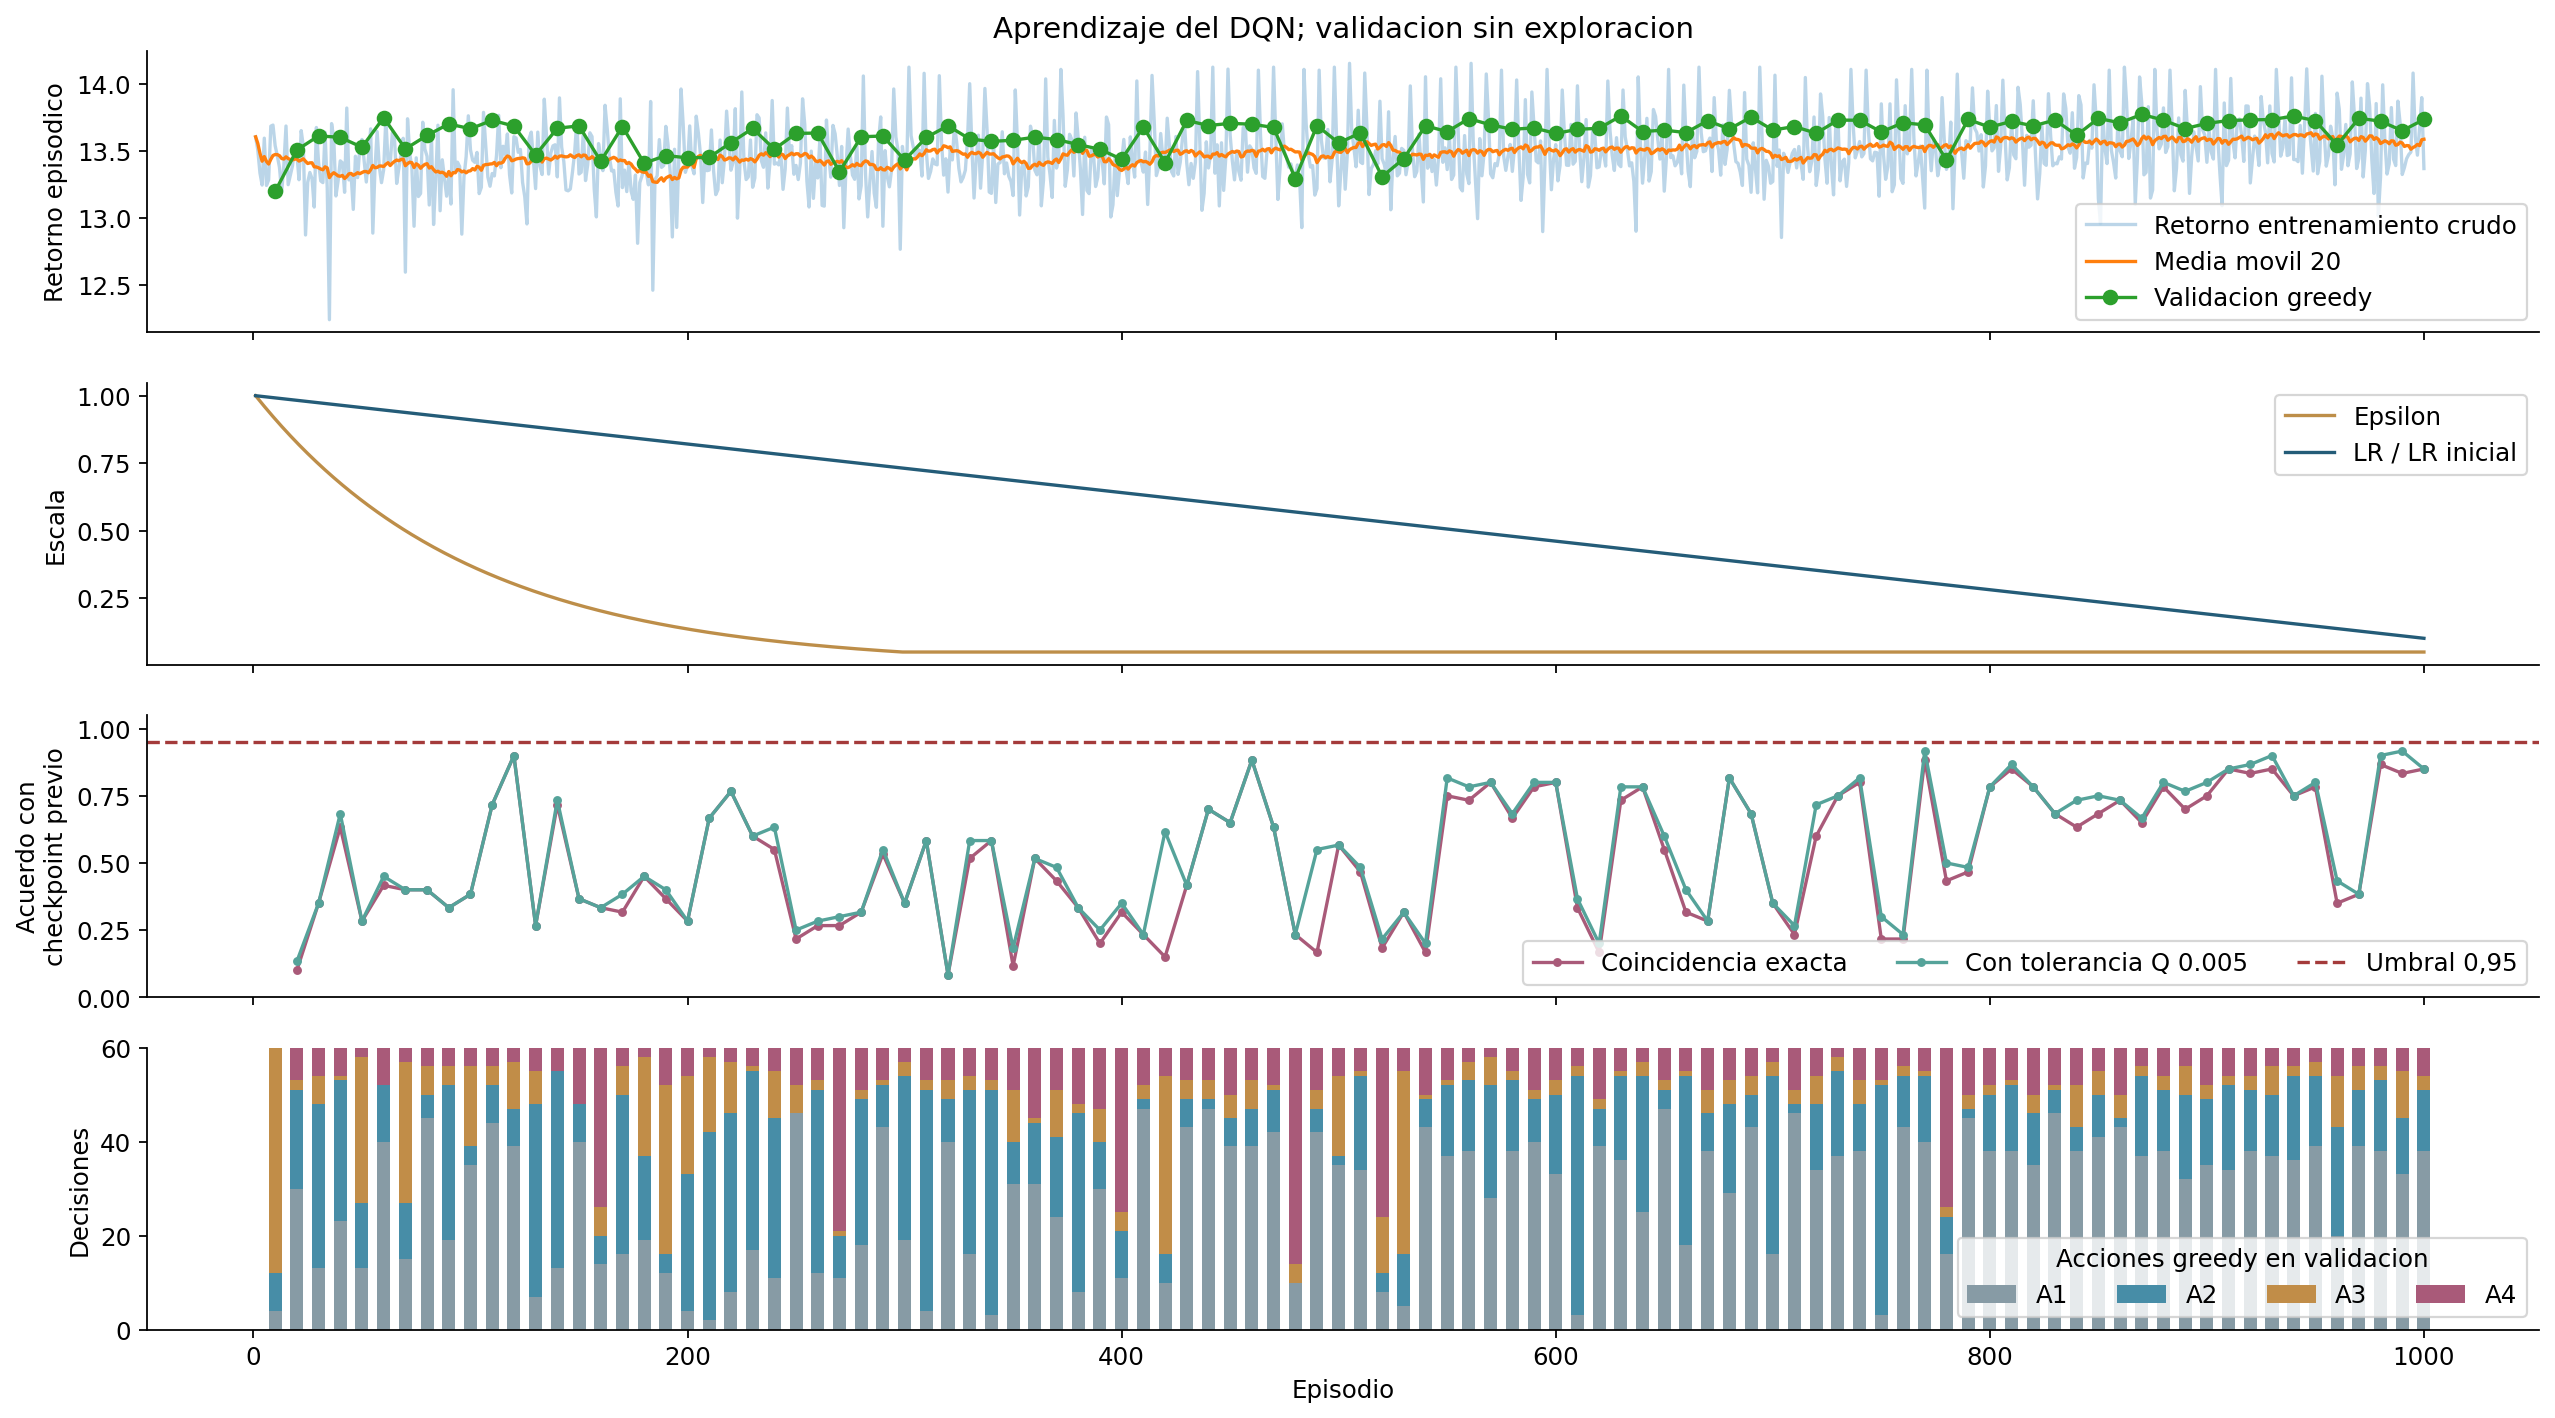
\includegraphics[width=0.52\textwidth,height=3.9cm,keepaspectratio]{kaggle/dqn-dummy/v4/outputs/figures/04_entrenamiento_retorno_epsilon.png}
\captionof{figure}{El retorno greedy se estabiliza antes que las acciones: el acuerdo exacto (panel 3) no llega al umbral rojo de 0,95 en los checkpoints finales.}
\end{center}

\vspace{-2pt}
{\scriptsize\textbf{Fuentes:} \texttt{main.ipynb}; CSV en
\texttt{kaggle/dqn-dummy/v4/outputs/}; figuras de auditoría en
\texttt{kaggle/dqn-dummy/v4/outputs/analisis/}. El documento enlazado
\texttt{C:/Users/jeffr/GitHub/tesis-darl/plan/diagnostico\_a3\_v4.md} no está
disponible en este equipo; conclusiones verificadas contra artefactos locales.}

\end{document}
